%%%%%%%%%%%%%%%%%%%%%%%%%%%%%%%%%%%%%%%%%%%%%%%%%%%%%%%%%%%%%%%%%%%%%%%%
%     LaTeX source code to approximate a NIST Technical report
%	  Instructions for authors: tinyurl.com/techpubsnist 
%	DOI watermark will be added on final PDF
% 	Developed by K. Miller, kmm5@nist.gov 
%	Last updated: 22-March-2019
%%%%%%%%%%%%%%%%%%%%%%%%%%%%%%%%%%%%%%%%%%%%%%%%%%%%%%%%%%%%%%%%%%%
\documentclass[12pt]{article}
\usepackage{amsmath}
\usepackage{amsfonts}   % if you want the fonts
\usepackage{amssymb}    % if you want extra symbols
\usepackage{graphicx}   % need for figures
\usepackage{xcolor}
\usepackage{bm}
\usepackage{secdot}		
\usepackage{mathptmx}
\usepackage{float}
\usepackage[utf8]{inputenc}
\usepackage{textcomp}
\usepackage[hang,flushmargin,bottom]{footmisc} % footnote format
\usepackage{longtable}
\usepackage{hhline}

\usepackage{titlesec}
\titleformat{\section}{\normalsize\bfseries}{\thesection.}{1em}{}	% required for heading numbering style
\titleformat*{\subsection}{\normalsize\bfseries}

\usepackage{tocloft}	% change typeset, titles, and format list of appendices/figures/tables
\renewcommand{\cftdot}{}	
\renewcommand{\contentsname}{Table of Contents}
\renewcommand{\cftpartleader}{\cftdotfill{\cftdotsep}} % for parts
\renewcommand{\cftsecleader}{\cftdotfill{\cftdotsep}}
\renewcommand\cftbeforesecskip{\setlength{4pt}{}}
\addtolength{\cftfignumwidth}{1em}
\renewcommand{\cftfigpresnum}{\figurename\ }
\addtolength{\cfttabnumwidth}{1em}
\renewcommand{\cfttabpresnum}{\tablename\ }
\setlength{\cfttabindent}{0in}    %% adjust as you like
\setlength{\cftfigindent}{0in} 

\usepackage{enumitem}         % to control spacing between bullets/numbered lists

%%%%% AUTHORS - PLACE YOUR OWN COMMANDS HERE %%%%%
\newcommand{\xray}{\hbox{X-ray}}  %box words
\newcommand{\lx}{L_{\rm X}}
\newcommand{\lbol}{L_{\rm AGN,bol}}
\newcommand{\mbh}{M_{\rm BH}}
\newcommand{\mstar}{M_{\star}}
\newcommand{\ox}{\alpha_{\rm ox}}
\newcommand{\ang}{\textup{\AA}}
\newcommand{\luv}{L_{2500 \ang}}
\newcommand{\luvx}{L_{2500 \ang, \rm X}}
\newcommand{\luvnox}{L_{2500 \ang, \rm noX}}
\newcommand{\fracA}{{\rm frac_{AGN}}}
\newcommand{\fracAx}{{\rm frac_{AGN, Xup}}}
\newcommand{\fracAnox}{{\rm frac_{AGN, noX}}}
\newcommand{\lxr}{L_{\rm 2 keV}}
\newcommand{\xcig}{{\sc \hbox{cigale}}}
\newcommand{\redchi}{\chi^2_{\rm red}}
% space telescopes
\newcommand{\hst}{{\it HST\/}}       
\newcommand{\herschel}{{\it Herschel\/}}
\newcommand{\chandra}{{\it Chandra\/}}
\newcommand{\rxte}{{\it RXTE\/}}
\newcommand{\rosat}{{\it ROSAT\/}}
\newcommand{\xmm}{\hbox{\it XMM-Newton\/}}
\newcommand{\nustar}{{\it NuSTAR\/}}
\newcommand{\athena}{{\it Athena\/}}
\newcommand{\jwst}{{\it JWST\/}}
\newcommand{\spitzer}{{\it Spitzer\/}}
\newcommand{\galex}{{\it GALEX\/}}
\newcommand{\swift}{{\it Swift\/}}
\newcommand{\akari}{{\it AKARI\/}}
\newcommand{\erosita}{{\it eROSITA\/}}
% Journals
\newcommand{\apj}{ApJ}
\newcommand{\aj}{AJ}
\newcommand{\apjs}{ApJS}
\newcommand{\apjl}{ApJL}
\newcommand{\aap}{A\&A}
\newcommand{\mnras}{MNRAS}
\newcommand{\nat}{Nature}
\newcommand{\araa}{ARA\&A}
\newcommand{\aapr}{A\&ARv}


\usepackage[]{natbib} % format bibliography 
\renewcommand{\bibsection}{}
\setlength{\bibsep}{0.0pt}

\usepackage[hidelinks]{hyperref}
\hypersetup{
	colorlinks = true,
urlcolor ={blue},
citecolor = {.},
linkcolor = {blue},
anchorcolor = {.},
filecolor = {.},
menucolor = {.},
runcolor = {.}
pdftitle={},
pdfsubject={},
pdfauthor={},
pdfkeywords={}
}
\urlstyle{same}

\usepackage{epstopdf} % converting EPS figure files to PDF

\usepackage{fancyhdr, lastpage}	% formatting document, calculating number of pages, formatting headers
\setlength{\topmargin}{-0.5in}
\setlength{\headheight}{39pt}
\setlength{\oddsidemargin}{0.25in}
\setlength{\evensidemargin}{0.25in}
\setlength{\textwidth}{6.0in}
\setlength{\textheight}{8.5in}

\usepackage{caption} % required for Figure labels
\captionsetup{font=small,labelfont=bf,figurename=Fig.,labelsep=period,justification=raggedright} 

%%%%%%%%%%% !!!!!! REQUIRED - FILL OUT METADATA HERE !!!!!!!! %%%%%%%%%%%%%%
%  	Report Number - fill in Report Number sent to you (see info below)
%   DOI Statement - fill in DOI sent to you 
%   Month Year - fill in Month and Year of Publication
%%%%%%%%%%%%%%%%%%%%%%%%%%%%%%%%%%%%%%%%%%%%%%%%%%%%%%%%%%%%%%%%%%%%%%%%%%%%%%%%%%%%%%
\newcommand{\pubnumber}{XXXX}
\newcommand{\DOI}{https://doi.org/10.6028/NIST.HB.XXXX}
\newcommand{\monthyear}{Month Year}
%%%%%%%%%%%%%%%%%%%%%%%%%%%%%%%%%%%%%%%%%%%%%%%%%%%%%%%%%%%%%%%%%%%%
%   	BEGIN DOCUMENT 
%%%%%%%%%%%%%%%%%%%%%%%%%%%%%%%%%%%%%%%%%%%%%%%%%%%%%%%%%%%%%%%%%%%%
\begin{document}
	\urlstyle{rm} % Format style of \url   

%%%%%%%%%%%%%%%%%%%%%%%%%%%%%%%%%%%%%%%%%%%%%%%%%%%%%%%%%%%%%%%%%%%%
%   Cover Page is REQUIRED and must contain the information 
%	displayed here, at a minimum. Additional artwork may be included 
%	(e.g., official project/conference logo, etc.).
%	Pub Number automated based on metadata
%%%%%%%%%%%%%%%%%%%%%%%%%%%%%%%%%%%%%%%%%%%%%%%%%%%%%%%%%%%%%%%%%%%%
\begin{titlepage}
\begin{flushright}
%%%%%%%%%%%%%%%%%%%%%%%%%%%%%%%%%%%%%%%%%%%%%%%%%%%%%%%%%%%%%%%%%%%%
% 	Automated based on metadata - delete if not applicable
%%%%%%%%%%%%%%%%%%%%%%%%%%%%%%%%%%%%%%%%%%%%%%%%%%%%%%%%%%%%%%%%%%%%
\LARGE{\textbf{}}\\
\vfill
%%%%%%%%%%%%%%%%%%%%%%%%%%%%%%%%%%%%%%%%%%%%%%%%%%%%%%%%%%%%%%%%%%%%
%	Title 
%%%%%%%%%%%%%%%%%%%%%%%%%%%%%%%%%%%%%%%%%%%%%%%%%%%%%%%%%%%%%%%%%%%%
\Huge{\textbf{CIGALE Manual (v1.0)}}\\
    \vfill
%%%%%%%%%%%%%%%%%%%%%%%%%%%%%%%%%%%%%%%%%%%%%%%%%%%%%%%%%%%%%%%%%%%%
%	Authors - add complete list of authors, affiliations will be 
%   added on title page
%%%%%%%%%%%%%%%%%%%%%%%%%%%%%%%%%%%%%%%%%%%%%%%%%%%%%%%%%%%%%%%%%%%%
    \large Yang, Guang (\url{gyang206265@gmail.com})\\
    \large Burgarella, Denis (\url{denis.burgarella@lam.fr})\\
\vfill
%%%%%%%%%%%%%%%%%%%%%%%%%%%%%%%%%%%%%%%%%%%%%%%%%%%%%%%%%%%%%%%%%%%%
%	The DOI is automated based on metadata.	
%%%%%%%%%%%%%%%%%%%%%%%%%%%%%%%%%%%%%%%%%%%%%%%%%%%%%%%%%%%%%%%%%%%%
\normalsize This manual (along with supplementary material) is available from:\\
\url{https://cigale.lam.fr/documentation/} \\
\vfill
%%%%%%%%%%%%%%%%%%%%%%%%%%%%%%%%%%%%%%%%%%%%%%%%%%%%%%%%%%%%%%%%%%%%
%	NIST LOGO - keep as-is
%%%%%%%%%%%%%%%%%%%%%%%%%%%%%%%%%%%%%%%%%%%%%%%%%%%%%%%%%%%%%%%%%%%%

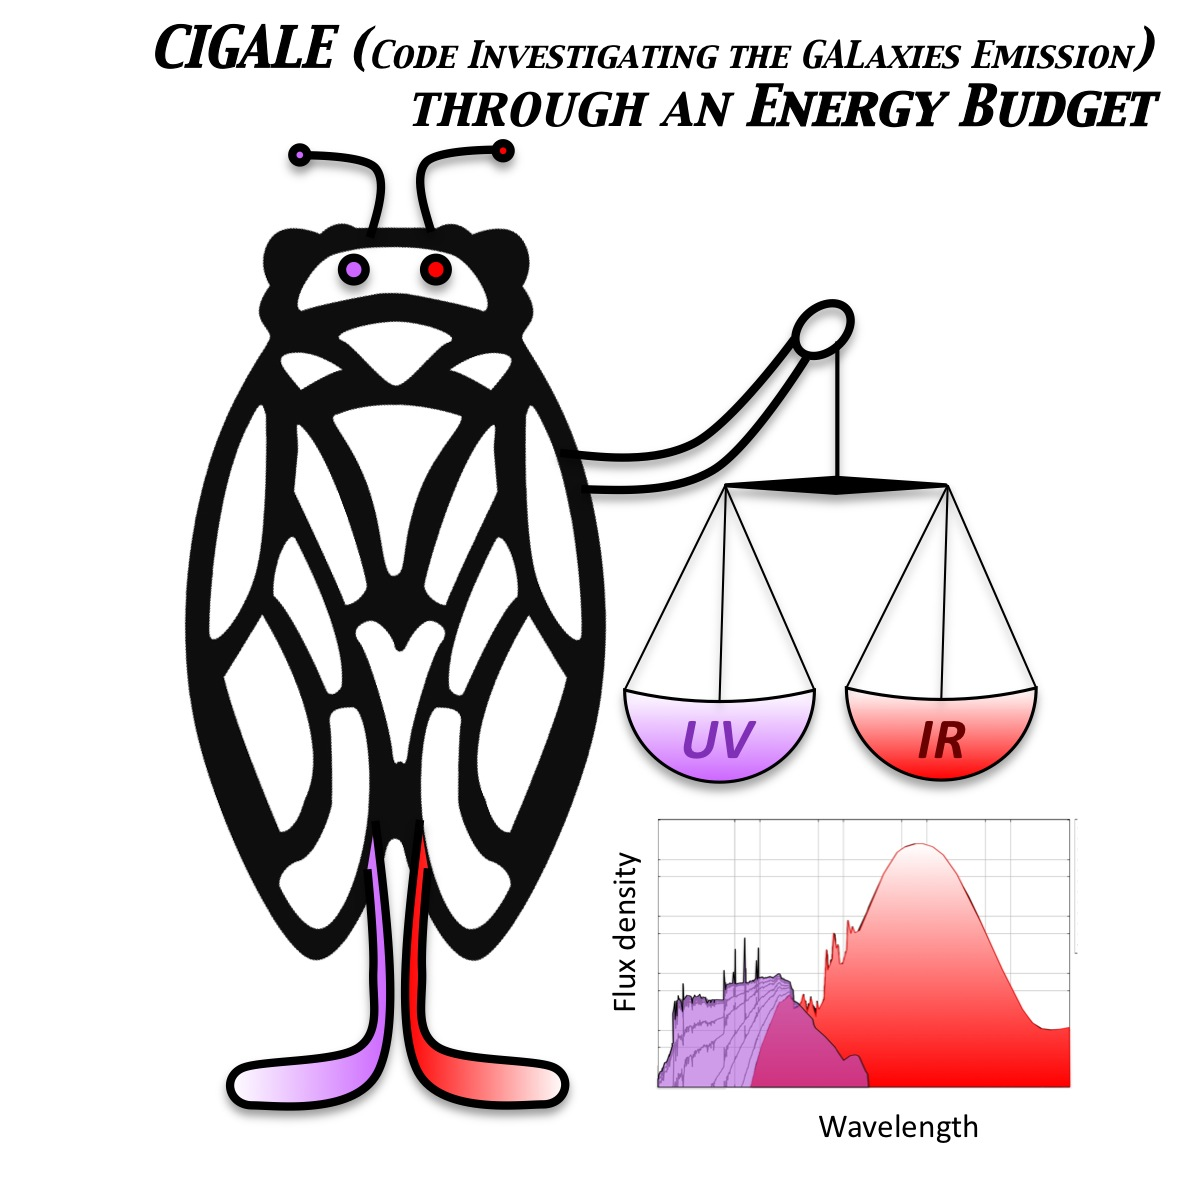
\includegraphics[width=0.5\linewidth]{CIGALE_Logo.jpg}\\ 
 
  
\end{flushright}
\end{titlepage}

%%%%%%%%%%%%%%%%%%%%%%%%%%%%%%%%%%%%%%%%%%%%%%%%%%%%%%%%%%%%%%%%%%%%
%   Table of Contents is required
% 	List of Tables & Figures required if more than 5 tables/figures
%%%%%%%%%%%%%%%%%%%%%%%%%%%%%%%%%%%%%%%%%%%%%%%%%%%%%%%%%%%%%%%%%%%%
\begin{center}
\tableofcontents
\listoftables
\listoffigures
\end{center}
\pagebreak

%%%%%%%%%%%%%%%%%%%%%%%%%%%%%%%%%%%%%%%%%%%%%%%%%%%%%%%%%%%%%%%%%%%%
%   Start body of text - page number starts with "1"
%%%%%%%%%%%%%%%%%%%%%%%%%%%%%%%%%%%%%%%%%%%%%%%%%%%%%%%%%%%%%%%%%%%%
\section{Overview}\label{sec:overview}
Code Investigating GALaxy Emission ({\sc cigale}) is a Python code for the fitting of spectral energy distribution (SED) of galaxies. 
It has been developed for more than 1.5 decades \citep[e.g.][]{burgarella05, noll09, serra11, roehlly14, boquien19}. 
The detailed algorithm is described in \cite{boquien19}.
\cite{yang20} upgraded \xcig\ to allow it fitting X-ray data, and this version is dubbed as ``{\sc x-cigale}''.
We further merged {\sc x-cigale} into the main branch of \xcig\ as well as implemented many improvements and functionalities \citep{yang22}.
The new version is marked as v2022.0.
This manual serves as a ``quick and practical'' reference for the user.
Further questions can be asked in our discussion forum (\url{https://github.com/mboquien/cigale/discussions}).
All materials of \xcig\ (including this manual) can be found on \url{https://cigale.lam.fr}.

In \S\ref{sec:install}, we describe the installation procedures.
\xcig\ has two working modes.
One is fitting the observed galaxy SEDs, and the other is simulating model SEDs. 
These two modes are described in \S\ref{sec:pdf} and \S\ref{sec:saveflux}, respectively. 
Appendix~\hyperref[app:par]{A} lists the main model parameters.
Appendix~\hyperref[app:file]{B} describes the supplementary files used in this manual. 
%Appendix~\ref{app:faq} includes the frequently asked questions.



\section{Installation}\label{sec:install}
The easiest way is to use pip installation.
To do this, in the downloaded \xcig\ directory,
simply run \\
\$ \textit{pip install .} \\

However, the pip installation above only allows you to use the default downloaded code. 
If you want to modify the code to serve your own research interest, you can install from source. 
The instruction is detailed at \url{https://github.com/mboquien/cigale/discussions/2}

%We assume you have Python 3.4 or higher working on your computer.
%We recommend using ANACONDA to install Python~3 (\url{https://www.anaconda.com/distribution/}).

%\subsection{Method I: pip}
%\begin{enumerate}
%    \item Download the experimental wheel (.whl file) from \url{https://cigale.lam.fr/}
%    \item Open terminal and run \\
%        \$ \textit{pip install pcigale-2018.0.1-py3-none-any.whl} (or any other version of .whl file) \\
%         to install \xcig. You can delete the .whl file after installation.
%\end{enumerate}

%\subsection{Method II: from source}
%\begin{enumerate}
%    \item Download the source file from \url{https://gitlab.lam.fr/gyang/cigale/tree/xray} and decompress
%    \item Install dependencies. Open terminal and run:
%    \begin{itemize}
%        \item[\$] \textit{conda install astropy numpy scipy sqlite sqlalchemy matplotlib configobj}
%    \end{itemize}
%    \item \$ \textit{cd pcigale} (or whatever the name or the directory is)
%    \item If you want to add your own filters for the SED analysis or the creation of models in filters, it is the correct time to do so.
%          Just add your filters into the directory:./database\_builder/filters/.
%          A minimum list of filter transmissions is provided with the \xcig\ distribution downloaded.
%    \item \$ \textit{Python setup.py build} \\
%          Note that if you already have the pcigale/data/data.db file, you need to delete it before re-building.
%    \item \$ \textit{Python setup.py develop} \\
%            will install \xcig. 
%            Note that the pcigale directory should not be removed or \xcig\ will no longer works.
%\end{enumerate}
\section{Run -- Fitting Observed Data: the ``pdf\_analysis'' mode}\label{sec:pdf}
In this Section, we detail the procedures of fitting observed data.

\subsection{Data Preparation}
\label{sec:data}
The input data for fitting should be a ASCII table with the format of the following: \\

\begin{tabular}{ccccccc} 
\# id & redshift & filter1 & filter1\_err & filter2 & filter2\_err & ... \\ 
J175535.47+660959.0 & 1.22 &  1.091e-02 & 1.20e-03 & 1.533e-02 & 1.56e-03 & ... \\
19260817 & 3.12 &  9.325e-03 & 1.04e-03 & 4.107e-02 & 4.18e-03 & ... \\ \\
\end{tabular}

The first column is the name for each source. 
The second column is the redshift information. 
The entry can be set to negative is you want to \xcig\ to search for redshift, i.e. the ``photometric redshift'' mode. 
If the entry is set to 0, then the source is assumed to be at 10~pc. Note that an optional column, ``distance'' (in units of Mpc), can be inserted after the redshift column. 
If the distance column is provided, then it will be used in lieu of the distance computed from the redshift.
The following columns are fluxes and $1\sigma$ uncertainties 
in units of mJy (photometry) or W~m$^{-2}$ (emission line).
Note that ``filter1'', ``filter2'' ... should be the filter names in \xcig\ database. 
You can run \\
\$ \textit{pcigale-filters list} \\
in the terminal to list all of the existing filters. 
You can also create your own filter in an ASCII file in the following format: \\

\begin{tabular}{ll} 
\# filter1 \\
\# photon \\
\# some comments \\
1340.62 & 0.0000 \\
1350.49 & 0.1154 \\
1370.21 & 0.1765 \\
\\
\end{tabular}

The first line is the filter name. 
The second line tells the filter type, and can be ``energy'' or ``photon'', which determines the way flux is calculated.\footnote{See \url{http://svo2.cab.inta-csic.es/theory/fps/} for detailed formulas.}
The third line presents some explanatory comments. 
The following lines are ``wavelength'' (in \r{A}) and ``transmission''. 
To implement the filter in \xcig\ database, you can add the filter ASCII file to \xcig\ filter directory (pcigale/atabasebuilder/filters/) and re-build the code (see \S\ref{sec:install}). 
Another way is to run the following command in the terminal: \\
\$ \textit{pcigale-filters add filter\_file} \\

Aside from normal flux and error, \xcig\ can also deal with upper limit. 
Fig.~\ref{fig:flux_fluxerr} summarizes the way how \xcig\ deal with the input fluxes and errors.

\begin{figure}[ht]
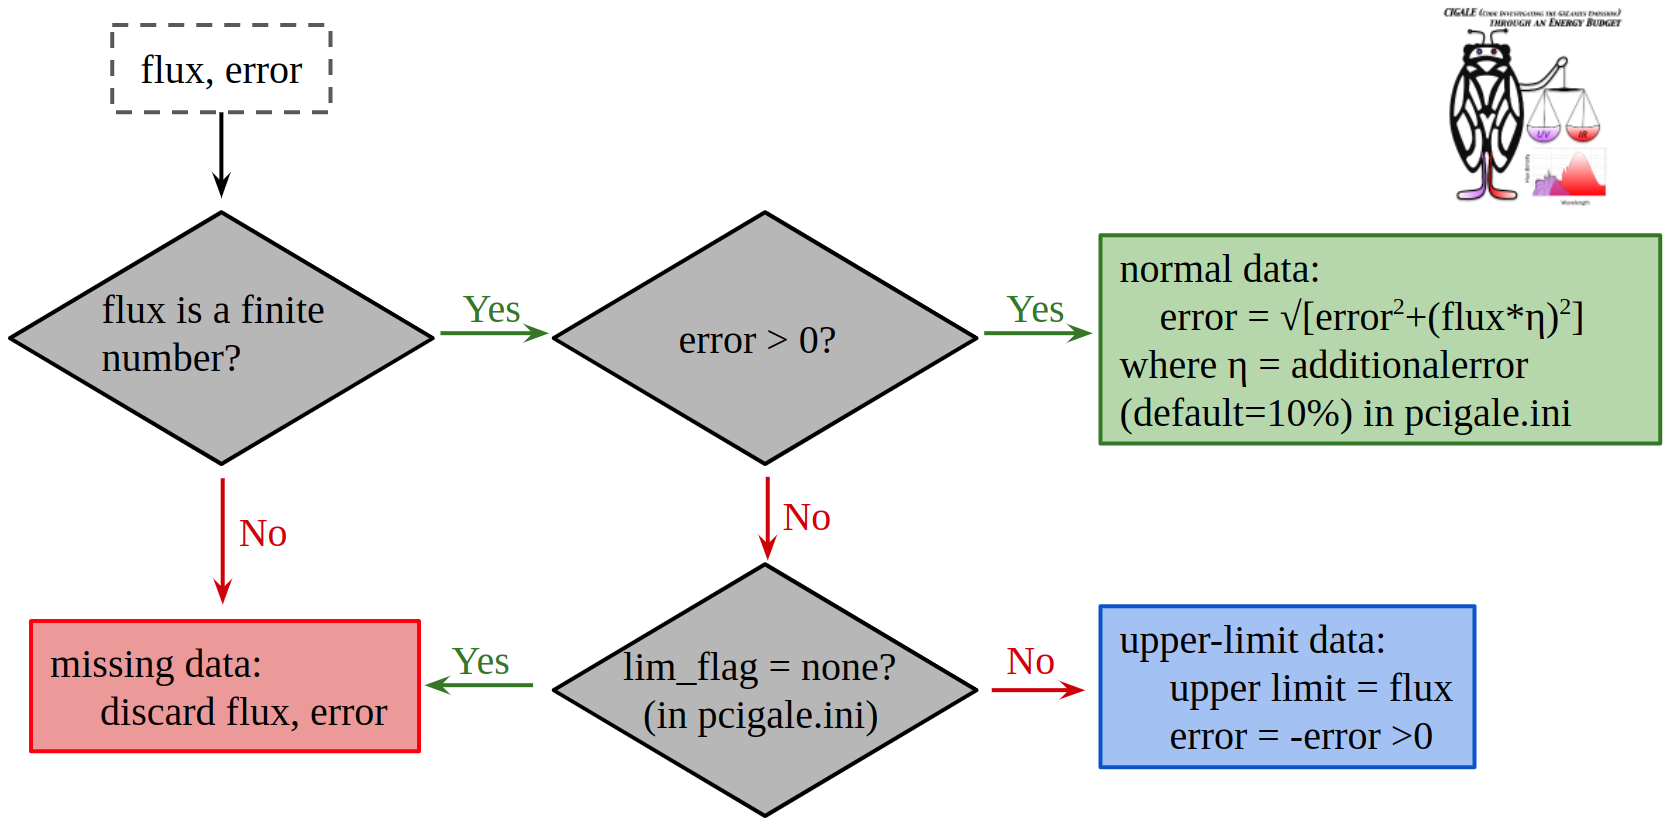
\includegraphics[width=\columnwidth]{pdfanalysis/flux_fluxerr.png}
\caption[How \xcig\ manages fluxes and flux errors]{This figure presents how \xcig\ manages (flux, error) for each filter.}
\label{fig:flux_fluxerr}
\end{figure}

\subsubsection{X-ray filters and fluxes}\label{sec:xray}
As explain in \cite{yang20}, \xcig\ requires that the input \xray\ fluxes are intrinsic.
This means that the energy-dependent instrumental response should have been corrected. 
Therefore, the \xray\ filters should be flat, i.e. boxcar-shaped. 
Fig.~\ref{fig:boxcar} presents an example \xray\ filter for 2--7~keV. 
\xcig\ includes a few filters for typical \xray\ bands. 
You can also create your own \xray\ filters. 
For your convenience, we provide a Python code (code/xray\_filter.py) to generate boxcar filters for a given \xray\ band. 
For example, you can run it as \\
\$ \textit{python} \\
$>>>$ \textit{import xray\_filter} \\
$>>>$ \textit{xray\_filter.write\_boxcar\_filter(``1to5.dat'', ``1to5'', 1, 5)} \\
will write a filter named ``1to5.dat'' for 1--5~keV. 

\begin{figure}[ht]
\centering
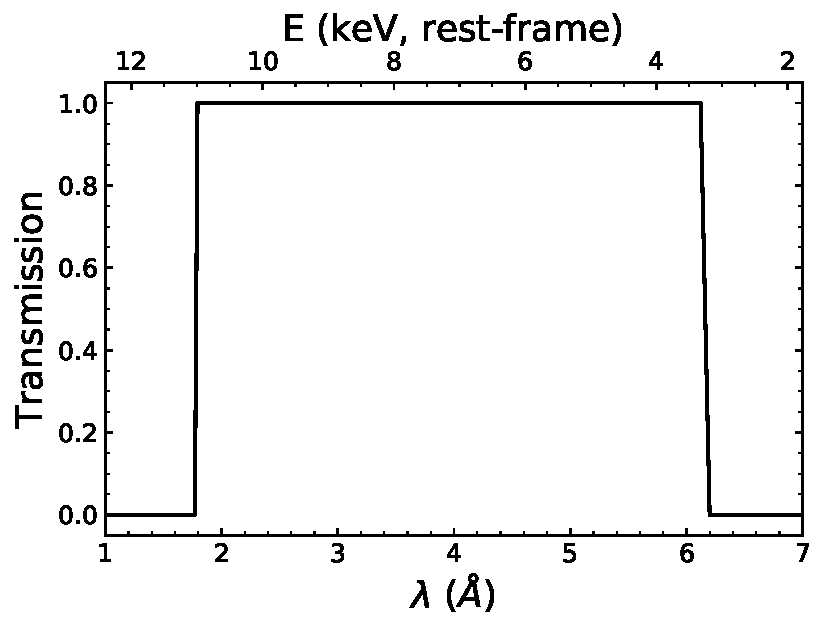
\includegraphics[width=0.6\columnwidth]{pdfanalysis/boxcar.pdf}
\caption[An example \xray\ boxcar filter for 2--7~keV]{An example \xray\ boxcar filter for 2--7~keV.}
\label{fig:boxcar}
\end{figure}

In \xray\ catalogs, the fluxes are often given in the cgs units of erg~s$^{-1}$~cm$^{-2}$. 
\xcig\ requires all inputs fluxes to be in units of mJy. 
Eq.~1 of \cite{yang20} gives the formula for the conversion. 
We also provide a Python code (``code/convert\_Fx.py'') to do this job. 
For example, \\
\$ \textit{python} \\
$>>>$ \textit{import convert\_Fx} \\
$>>>$ \textit{Fnu, Fnu\_err = convert\_Fx.convt\_Fx\_to\_Fnu([1e-16, 1e-15], [3e-17, 2e-16], 2, 7)} \\
will convert \hbox{2--7}~keV fluxes of [1e-16, 1e-15] erg~s$^{-1}$~cm$^{-2}$ and errors of [3e-17, 2e-16] erg~s$^{-1}$~cm$^{-2}$ to mJy fluxes (``Fnu'') and flux errors (``Fnu\_err''). 
These outputs of ``Fnu'' and ``Fnu\_err'' can then be written to \xcig\ input data.

\subsection{Configuration and Run}\label{sec:config}
Open terminal, cd to your working directory. \\
\$ \textit{pcigale init} \\
will initialize configuration files called ``pcigale.ini'' and ``pcigale.ini.spec''.
You only need to edit ``pcigale.ini''.
There are five parameters in this file (with many commentary words starting with \#): ``data\_file'', ``parameters\_file'', ``sed\_modules'', ``analysis\_method'', ``cores''. 
\begin{itemize}
    \item ``data\_file'' is the input data file (\S\ref{sec:data}). 
    \item ``parameters\_file'' is the optional file when simulating data (see \S\ref{sec:saveflux}). It should be  empty when fitting observed data. 
    \item ``sed\_modules'' lists the names of the SED modules that will be used in the run. 
    The available modules are listed in the commentary parts of the ``pcigale.ini'' file. 
    The module names should follow the order given in the commentary parts. 
    \item ``analysis\_method'' is \xcig\ mode. Should be ``pdf\_analysis'' for data-fitting purpose.
    \item ``cores'' is the number of CPU cores that will be used. Note that increasing the number of cores may not necessarily boost the speed. 
\end{itemize}
We provide two example runs of \hbox{AKARI-NEP} AGNs and SDSS QSOs \citep{yang20} along with this manual (``examples/akari\_nep\_xray\_agn'' and ``examples/sdss\_qso/''). 
In the test run, the configuration file reads:
\begin{itemize}
    \item[] \textit{data\_file = sdss\_qso.txt}
    \item[] \textit{parameters\_file = }
    \item[] \textit{sed\_modules = sfhdelayed, bc03, nebular, dustatt\_calzleit, dale2014, skirtor2016, xray, redshifting}
    \item[] \textit{analysis\_method = pdf\_analysis}
    \item[] \textit{cores = 4}
\end{itemize}
After setting the initial configuration file, run the following in terminal\\
\$ \textit{pcigale genconf} \\
which will generate the full configuration files ``pcigale.ini'' and ``pcigale.ini.spec''. 

Open ``pcigale.ini'', and you will find more parameters have been added. 
Following ``cores'', there are two parameters ``bands'' and ``properties''. 
You can see that \xcig\ already fills in the band and property names from the input data. 
But if you do not want to use some information, you can delete some entries.  

The other new parameters fall into two categorises, [sed\_modules\_params] and [analysis\_params]. 
[sed\_modules\_params] includes the configurations for each adopted SED module. 
These parameters should be self-explanatory, and we do not further explain them here. 
[sed\_modules\_params] determines the number of models that will be built. 
After finishing [sed\_modules\_params], you can check the number of models with \\
\$ \textit{pcigale check} \\
\textit{With this configuration cigale will compute 15966720 models.} \\

\noindent [analysis\_params] includes the configurations for the analysis, i.e.,
\begin{itemize}
    \item ``variables'' is the list of the physical properties to estimate in the Bayesian-like style. 
    The full list of properties can be found in Appendix~\hyperref[app:par]{A}.
    Note that this parameter only affects Bayesian results. 
    The best-fit (least-$\chi^2$) values for all properties are calculated in the results anyway.
    \item ``save\_best\_sed'' can be ``True'' or ``False''. 
    If ``True'', will save the best-fit SED and SFH models for each source. 
    \item ``save\_chi2'' can be ``none'', ``fluxes'', ``properties'', or ``all''. 
    If ``fluxes'', will save the raw $\chi^2$ for each photometric band for each source. 
    If ``properties'', will save $\chi^2$ for ``variables'' above for each source.
    If ``all'', will save $\chi^2$ for both photometric bands and ``variables''.
    If ``none'', will not save $\chi^2$.
    %The output files will be in {\sc numpy.memmap} format. 
    We provide a {\sc python} script ``code/read\_chi.py'' for reading the output $\chi^2$ file (in .npy format).
    \item ``lim\_flag'' can be ``none'' ``full'', or ``noscaling''. 
    If ``none'', will discard all upper limits in the input data (see Fig.~\ref{fig:flux_fluxerr}).
    If ``full'', will analyze upper limits using exact computation (slow speed). 
    If ``noscaling'' (default), will use an approximate method to deal with upper limits, which is a good balance between efficiency and reliability.
    \item ``mock\_flag'' can be ``True'' or ``False''.
    If ``True'', will create a mock catalog and analyze it. 
    This is a quick way to check if the physical properties can be constrained in a self-consistent way (see \S4.3 of \citealt{boquien19}).
    \item ``redshift\_decimals'' is the number of decimals to round the observed redshifts. 
    To disable rounding give a negative value.
    \item ``blocks'' is the number of blocks for the run.
    The default is 1, which is optimal for speed. 
    But if your computer memory is not enough, you can set it to $>1$. 
\end{itemize}
After completing ``pcigale.ini'', you can run \xcig\ with \\
\$ \textit{pcigale run} \\
Along with this manual, we provide an example configuration file, ``examples/sdss\_qso/pcigale.ini''.  

\subsection{Results}\label{sec:pdf_res}
After the run finishes, you can find the results in the ``out/'' directory. 
This directory contains:
\begin{itemize}
    \item ``results.txt'' (ASCII format) and ``results.fits'' (FITS format), the source-property catalog from the fitting.
    \item ``pcigale.ini'' and ``pcigale.ini.spec'', the used configuration files. 
    \item ``observations.txt'' and ``observations.fits'', the input observed data. 
    \item ``{SOURCE ID}\_best\_model.fits'' (exist if ``save\_best\_sed'' is set to ``True''), the best-fit SEDs for {SOURCE ID}, including the total and different components.
    \item ``{SOURCE ID}\_SFH.fits'' (exist if ``save\_best\_sed'' is set to ``True''), the best-fit SFH for {SOURCE ID}.
    \item ``{SOURCE ID}\_{PROPERTY}\_chi2-block-{BLOCK}.npy'' (exist if ``save\_chi2'' is set to ``True''), the raw $\chi^2$ of {PROPERTY} for {SOURCE ID} in {BLOCK}. 
    We provide a {\sc python} script to read these files (``code/read\_chi.py''). 
    \item ``mock\_observations.txt'', ``mock\_observations.fits'', ``results\_mock.txt'', and ``results\_mock.fits'' (exist if ``mock\_flag'' is set to ``True''), the mock catalog and fitting results. 
\end{itemize}
You can visualize the results with \textit{pcigale-plots} command. 
For example, \\
\$ \textit{pcigale-plots sed}\\
will generate the best-fit SED plot for each source in pdf format (``out/{SOURCE ID}\_best\_model.pdf'').
Fig.~\ref{fig:exm_sed} shows an example SED generated by the \textit{pcigale-plots} command.

\begin{figure}[ht]
\centering
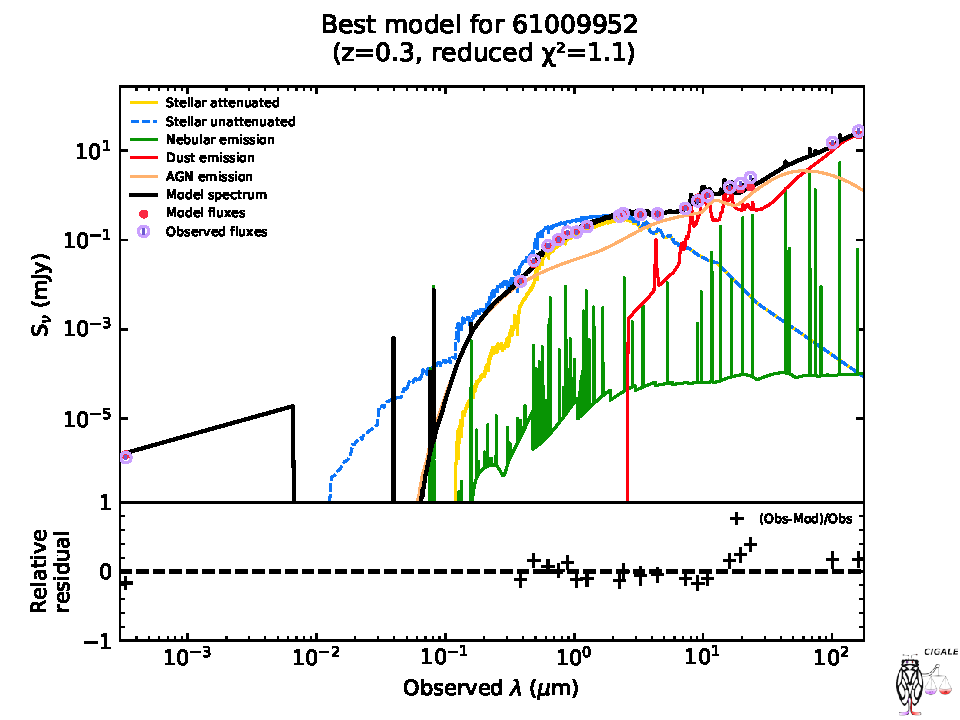
\includegraphics[width=\columnwidth]{pdfanalysis/exm_sed.pdf}
\caption[An example SED generated by the \textit{pcigale-plots} command]{An example SED generated by the \textit{pcigale-plots} command.}
\label{fig:exm_sed}
\end{figure}
\section{Run -- Simulating Data: the ``savefluxes'' mode}\label{sec:saveflux}
{\sc X-CIGALE} can not only fit the observed data, but also simulate data from a user-defined model set. 
In this section, we detail the simulation procedures. 

\subsection{Configurations and Run}\label{sec:mod}
Similar as in \S\ref{sec:config}, the first step is still the initialization of configuration files.
In your working directory, run \\
\$ \textit{pcigale init} \\
resulting ``pcigale.ini'' and ``pcigale.ini.spec''.
``pcigale.ini'' has five parameters, i.e.
\begin{itemize}
    \item ``data\_file'' is the input data file, should leave empty when simulating data.  
    \item ``parameters\_file'' is the optional file containing the list of physical parameters.
    Each column must be in the form module\_name.parameter\_name, with each line being a different model.
    If this file is given, then \xcig\ will neglect the parameters in [sed\_modules\_params]. 
    \item ``sed\_modules'' lists the names of the SED modules that will be used in the run. 
    The available modules are listed in the commentary parts of the ``pcigale.ini'' file. 
    The module names should follow the order given in the commentary parts. 
    \item ``analysis\_method'' is \xcig\ mode. Should be ``savefluxes'' for simulation purpose.
    \item ``cores'' is the number of CPU cores that will be used. Note that increasing the number of cores may not necessarily boost the speed. 
\end{itemize}
Along with this manual, we provide an example simulation run (``examples/simulate\_color'').
In the test run, the configuration file reads:
\begin{itemize}
    \item[] \textit{data\_file = }
    \item[] \textit{parameters\_file = }
    \item[] \textit{sed\_modules = sfhdelayed, bc03, nebular, dustatt\_calzleit, dale2014, redshifting}
    \item[] \textit{analysis\_method = savefluxes}
    \item[] \textit{cores = 4}
\end{itemize}
After setting the initial configuration file, run \\
\$ \textit{pcigale genconf} \\
which will generate the full configuration files ``pcigale.ini'' and ``pcigale.ini.spec''. 

As in \S\ref{sec:config}, you will have to edit ``pcigale.ini''. 
Similar in the data-fitting mode \S\ref{sec:pdf}, ``pcigale.ini'' has two new parameters, 
``bands'' and ``properties''.
You can key in your interested band and property names, which will appear in the result catalog after the run.
Other new parameters belong to [sed\_modules\_params] or [analysis\_params]. 
[sed\_modules\_params] has the same parameters as in the pdf\_analysis mode. 
Note that you must give ``redshfit'' values in the savefluxes mode, while you can leave it blank to use the redshift values in the input file in the pdf\_analysis mode.
[analysis\_params] only has three parameters, i.e.,
\begin{itemize}
    \item ``variables'' is the list of the model physical properties to appear in the results. 
    The full list of properties can be found in Appendix~\hyperref[app:par]{A}.
    You can leave it empty to include all available properties.
    \item ``save\_sed'' can be ``True'' or ``False''. 
    If ``True'', will save the best-fit SED and SFH models for each simulated source. 
    \item ``blocks'' is the number of blocks for the run.
    The default is 1, which is optimal for speed. 
    But if your computer memory is not enough, you can set it to an integer $\geq 2$. 
\end{itemize}

After finishing ``pcigale.ini'', you can run with \\
\$ \textit{pcigale run} \\
Along with this manual, we provide an example configuration file, ``examples/simulate\_bzk/pcigale.ini''.

\subsection{Results}
The results are still in the ``out/'' directory. 
This directory contains:
\begin{itemize}
    \item ``models-block-0.txt'' (ASCII format) and ``models-block-0.fits'' (FITS format), the simulated source-property catalog from the models.
    \item ``pcigale.ini'' and ``pcigale.ini.spec'', the used configuration files. 
    \item ``{MODEL ID}\_best\_model.fits'' (exist if ``save\_sed'' is set to ``True''), the model SEDs for {MODEL ID}, including the total and different components. 
    \item ``{MODEL ID}\_SFH.fits'' (exist if ``save\_sed'' is set to ``True''), the model SFH for {MODEL ID}.
\end{itemize}
Note that the extensive properties (e.g., stellar mass and star formation rate) have not been properly normalized in the results. 
You might want to normalize by, e.g., stellar mass or flux, before using these quantities. 

In our example (``examples/simulate\_bzk/''), we simulate the $BzK$ color-color diagram \citep{daddi04} as displayed in Fig.~\ref{fig:bzk}.

\begin{figure}[ht]
\centering
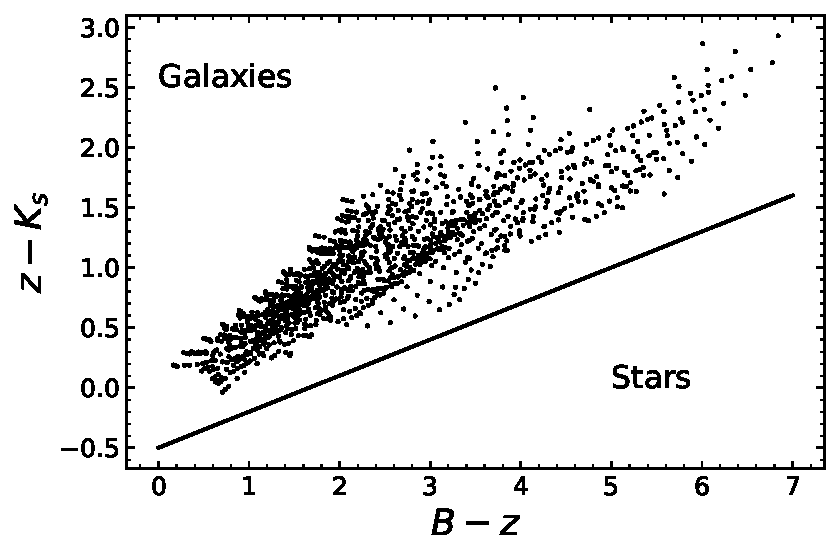
\includegraphics[width=\columnwidth]{savefluxes/bzk.pdf}
\caption[A $BzK$ diagram simulated in the savefluxes mode]{A $BzK$ diagram simulated in the savefluxes mode. 
The solid line indicates the empirical separation between galaxies and stars \citep{daddi04}.}
\label{fig:bzk}
\end{figure}



\section*{References}
\addcontentsline{toc}{section}{References}
\bibliographystyle{apj}
\bibliography{all.bib}

\section*{Appendix A: Model Parameters}
\label{app:par}
\addcontentsline{toc}{section}{Appendix A: Model Parameters}
The main parameters that can be analysed are listed below (see ``pcigale.ini'' and the output catalog for a full list of parameters)
The free parameters that can be set directly in the ``pcigale.ini'' file are highlighted in blue. 

If you wish to estimate the physical parameters in logarithmic, you only have to add ``\_log'' at the end of the name of the parameter, e.g., sfh.burst\_age will become sfh.burst\_age\_log
and... le tour est jou\'e!

%\begin{table}[h] 
%\centering
\begin{longtable}{| p{.20\textwidth} | p{.40\textwidth} | p{.40\textwidth} |} 
\caption[Physical parameters in \xcig]{Physical parameters in \xcig. Free parameters are highlighted in blue.} \\ % needs to go inside longtable environment
\hline
Module & Parameter & Description \\ \hline
sfh2exp & \textcolor{blue}{sfh.tau\_main}  & e-folding [Myr] time of the main stellar population model \\ \hline
...     & \textcolor{blue}{sfh.tau\_burst} & e-folding [Myr] time of the late starburst population model \\ \hline
...     & \textcolor{blue}{sfh.f\_burst}   & Mass fraction of the late burst population (0 to 1) \\ \hline
...     & \textcolor{blue}{sfh.burst\_age} & Age [Myr] for the burst \\ \hline
...     & \textcolor{blue}{sfh.age}        & Age [Myr] of the oldest stars in the galaxy \\ \hline
...     & sfh.sfr                          & Instantaneous star formation rate \\ \hline
...     & sfh.sfr10Myrs                    & Star formation rate averaged over 10 Myrs \\ \hline
...     & sfh.sfr100Myrs                   & Star formation rate averaged over 100 Myrs \\ \hline
...     & sfh.integrated                   & Star formation rate integrated from the star formation history \\ \hline
sfhdelayed & \textcolor{blue}{sfh.tau\_main} & e-folding [Myr] time of the main stellar population model \\ \hline
...        & \textcolor{blue}{sfh.age}       & Age [Myr] of the oldest stars in the galaxy \\ \hline
...     & sfh.sfr                            & Instantaneous star formation rate \\ \hline
...     & sfh.sfr10Myrs                      & Star formation rate averaged over 10 Myrs \\ \hline
...     & sfh.sfr100Myrs                     & Star formation rate averaged over 100 Myrs \\ \hline
...     & sfh.integrated                     & Star formation rate integrated from the star formation history \\ \hline
sfhperiodic & \textcolor{blue}{sfh.delta\_bursts} & Elapsed time between the beginning of each burst in Myr. \\ \hline
...         & \textcolor{blue}{sfh.tau\_bursts}   & Duration (rectangle) or e-folding time of all short events in Myr. \\ \hline
...         & sfh.integrated                      & Star formation rate integrated from the star formation history \\ \hline
sfhfromfile & \textcolor{blue}{sfh.id} & id of the input SFH \\ \hline
...         & sfh.sfr                  & Instantaneous star formation rate \\ \hline
...         & sfh.sfr10Myrs            & Star formation rate averaged over 10 Myrs \\ \hline
...         & sfh.sfr100Myrs           & Star formation rate averaged over 100 Myrs \\ \hline
...         & sfh.integrated           & Star formation rate integrated from the star formation history \\ \hline 
m2005       & \textcolor{blue}{stellar.imf}                         & IMF of the stellar model \\ \hline
...         & \textcolor{blue}{stellar.metallicity}                 & Metallicity of the stellar model \\ \hline
...         & \textcolor{blue}{stellar.old\_young\_separation\_age} & Age of the separation old/young stars \\ \hline
...         & stellar.mass\_total\_old                              & Stellar mass of old stars \\ \hline
...         & stellar.mass\_alive\_old                              & Stellar mass of old stars alive \\ \hline
...         & stellar.mass\_total\_young                            & Stellar mass of young stars \\ \hline
...         & stellar.mass\_alive\_young                            & Stellar mass of young stars alive \\ \hline
...         & stellar.mass\_total                                   & Total stellar mass of stars \\ \hline
...         & stellar.mass\_alive                                   & Total stellar mass alive \\ \hline
bc03        & \textcolor{blue}{stellar.imf}                         & IMF of the stellar model \\ \hline
...         & \textcolor{blue}{stellar.metallicity}                 & Metallicity of the stellar model \\ \hline
...         & \textcolor{blue}{stellar.old\_young\_separation\_age} & Age of the separation old/young stars \\ \hline
...         & stellar.m\_star\_young                                & Stellar mass of young stellar population \\ \hline
...         & stellar.n\_ly\_young                                  & Number of Ly continuum photons from young stellar population \\ \hline
...         & stellar.m\_star\_old                                  & Stellar mass of old stellar population \\ \hline
...         & stellar.n\_ly\_old                                    & Number of Ly continuum photons from old stellar population \\ \hline
...         & stellar.m\_star                                       & Total mass of stars \\ \hline
nebular & \textcolor{blue}{nebular.f\_esc}  & Fraction of Lyman continuum photons escaping the galaxy \\ \hline
...     & \textcolor{blue}{nebular.f\_dust} & Fraction of Lyman continuum photons absorbed by dust \\ \hline
...     & \textcolor{blue}{nebular.logU}    & Ionisation parameter \\ \hline
dustatt\_calzleit    & \textcolor{blue}{attenuation.uv\_bump\_amplitude}  & Amplitude of the UV bump. For the Milky Way: 3 \\ \hline
...                  & \textcolor{blue}{attenuation.powerlaw\_slope}      & Slope delta of the power law modifying the attenuation curve \\ \hline
...                  & \textcolor{blue}{attenuation.E\_BVs.stellar.young} & E(B-V) of the young stellar population. Note that E(B-V) is an internal parameter which does not correspond to E(B-V) except for the exact calzetti law (delta=0), E(B-V)= $A_B -A_V$ should be calculated by the user. \\ \hline
...                  & \textcolor{blue}{attenuation.ebvs\_old\_factor}    & Reduction factor of E(B-V) for the old population compared to the young one \\ \hline
...                  & attenuation.E\_BVs.stellar.old & E(B-V) of the old stellar population. Note that E(B-V) is an internal parameter which does not correspond to E(B-V) except for the exact calzetti law (delta=0), E(B-V)= $A_B -A_V$ should be calculated by the user.  \\ \hline
...                  & attenuation.(filter)                               & Attenuation in a given filter. This filter (e.g., FUV, B, V,...) must be provided to \xcig. \\ \hline 
dustatt\_powerlaw & \textcolor{blue}{attenuation.uv\_bump\_amplitude}  & Amplitude of the UV bump. For the Milky Way: 3 \\ \hline
...               & \textcolor{blue}{attenuation.powerlaw\_slope}      & Slope delta of the power law modifying the attenuation curve \\ \hline
...               & \textcolor{blue}{attenuation.Av.stellar.young}     & V-band attenuation of the young population \\ \hline
...               & \textcolor{blue}{attenuation.av\_old\_factor}      & Reduction factor of $A_V$ for the old population compared to the young one \\ \hline        
...               & attenuation.Av.stellar.young                       & V-band attenuation of the old population \\ \hline
...               & attenuation.(filter)                               & Attenuation in a given filter. This filter (e.g., FUV, B, V,...) must be provided to \xcig \\ \hline 
dl2014 & \textcolor{blue}{dust.umin}  & Parameter U\_min in \cite{draine07} templates \\ \hline
...    & \textcolor{blue}{dust.alpha} & Parameter alpha\_max in \cite{draine07} templates \\ \hline
...    & \textcolor{blue}{dust.gamma} & Parameter gamma in \cite{draine07} templates \\ \hline 
...    & \textcolor{blue}{dust.qpah}  & Parameter q$_{\rm PAH}$ in \cite{draine14} updated templates \\ \hline
...    & dust.luminosity              & Estimated dust luminosity using an energy balance \\ \hline
dale2014 & \textcolor{blue}{agn.fracAGN\_dale2014} & AGN fraction. Note that the AGN is a type 1 \\ \hline
...      & \textcolor{blue}{dust.alpha}            & Parameter alpha$_{\rm max}$ in \cite{dale14} templates \\ \hline
...      & dust.luminosity                         & Estimated dust luminosity using an energy balance \\ \hline
fritz2006 & \textcolor{blue}{agn.gamma}            & Parameter gamma in \cite{fritz06} \\ \hline
...       & \textcolor{blue}{agn.opening\_angle}   & Full opening angle of the dust torus (Fig 1 of \cite{fritz06}) \\ \hline
...       & \textcolor{blue}{agn.psy}              & Angle between AGN axis and line of sight \\ \hline
...       & \textcolor{blue}{agn.fracAGN}          & Fraction of AGN IR luminosity to total IR luminosity \\ \hline
...       & \textcolor{blue}{agn.r\_ratio}         & Ratio of the maximum to minimum radii of the dust torus \\ \hline
...       & \textcolor{blue}{agn.tau}              & Torus optical depth at 9.7 microns \\ \hline
...       & \textcolor{blue}{agn.beta}             & Parameter beta in \cite{fritz06} \\ \hline
...       & \textcolor{blue}{agn.law}              & The extinction law of polar dust: 0 (SMC), 1 \cite{calzetti00}, or 2 \cite{gaskell04} \\ \hline
...       & \textcolor{blue}{agn.EBV}              & E(B-V) for extinction in polar direction \\ \hline
...       & \textcolor{blue}{agn.temperature}      & Temperature of the polar dust in K \\ \hline
...       & \textcolor{blue}{agn.emissivity}       & Emissivity index of the polar dust \\ \hline
...       & agn.disk\_luminosity                   & The AGN disc luminosity (might be extincted) \\ \hline
...       & agn.therm\_luminosity                  & The AGN dust reemitted luminosity \\ \hline
...       & agn.scatt\_luminosity                  & The AGN scattered luminosity \\ \hline
...       & agn.luminosity                         & The sum of agn.disk\_luminosity, agn.therm\_luminosity, and agn.scatt\_luminosity \\ \hline
...       & agn.intrin\_Lnu\_2500A                 & The intrinsic AGN $L_\nu$ at 2500~\AA\ \\ \hline
...       & agn.accretion\_power                   & The intrinsic AGN disk luminosity averaged over all directions \\ \hline
skirtor2016 & \textcolor{blue}{agn.t}           & Average edge-on torus optical depth at 9.7 micron \\ \hline
...         & \textcolor{blue}{agn.pl}          & Power-law exponent that sets radial gradient of dust density \\ \hline
...         & \textcolor{blue}{agn.q}           & Index that sets dust density gradient with polar angle \\ \hline
...         & \textcolor{blue}{agn.oa}          & Angle measured between the equatorial plan and edge of the torus \\ \hline
...         & \textcolor{blue}{agn.R}           & Ratio of outer to inner radius, R\_out/R\_in \\ \hline
...         & \textcolor{blue}{agn.i}           & Viewing angle. i=[0, 90$^\circ$-oa): face-on, type 1 view; i=[90$^\circ$-oa, 90$^\circ$]: edge-on, type 2 view \\ \hline
...         & \textcolor{blue}{agn.fracAGN}     & Fraction of AGN IR luminosity to total IR luminosity \\ \hline
...         & \textcolor{blue}{agn.law}         & The extinction law of polar dust: 0 (SMC), 1 \cite{calzetti00}, or 2 \cite{gaskell04} \\ \hline
...         & \textcolor{blue}{agn.EBV}         & E(B-V) for extinction in polar direction \\ \hline
...         & \textcolor{blue}{agn.temperature} & Temperature of the polar dust in K \\ \hline
...         & \textcolor{blue}{agn.emissivity}  & Emissivity index of the polar dust \\ \hline
...         & agn.disk\_luminosity              & The observed AGN disc luminosity (might be extincted) \\ \hline
...         & agn.dust\_luminosity              & The observed AGN dust reemitted luminosity \\ \hline
...         & agn.luminosity                    & The sum of agn.disk\_luminosity and agn.dust\_luminosity \\ \hline
...         & agn.intrin\_Lnu\_2500A            & The intrinsic AGN $L_\nu$ at 2500~\AA\ at viewing angle $=30^\circ$ \\ \hline
...         & agn.accretion\_power              & The intrinsic AGN disk luminosity averaged over all directions \\ \hline
xray & \textcolor{blue}{xray.gam}                 & The photon index (Gamma) of AGN intrinsic X-ray spectrum \\ \hline
...  & \textcolor{blue}{xray.max\_dev\_alpha\_ox} & Maximum deviation from the $\ox$-$\luv$ relation in \cite{just07} \\ \hline
...  & \textcolor{blue}{xray.gam\_lmxb}           & The photon index of AGN low-mass X-ray binaries \\ \hline
...  & \textcolor{blue}{xray.gam\_hmxb}           & The photon index of AGN high-mass X-ray binaries \\ \hline
...  & xray.agn\_Lnu\_2keV                        & The AGN $L_\nu$ at 2~keV \\ \hline
...  & xray.agn\_Lx\_2to10keV                     & The AGN 2--10~keV luminosity \\ \hline
...  & xray.agn\_Lx\_total                        & The AGN total (0.25--1200~keV) \xray\ luminosity \\ \hline
...  & xray.alpha\_ox                             & The AGN $\ox$ \\ \hline
...  & xray.lmxb\_Lx\_2to10keV                    & The 2--10~keV LMXB luminosity \\ \hline
...  & xray.hmxb\_Lx\_2to10keV                    & The 2--10~keV HMXB luminosity \\ \hline
...  & xray.hotgas\_Lx\_0p5to2keV                 & The 0.5--2~keV hot-gas luminosity \\ \hline
radio & \textcolor{blue}{radio\_qir}   & FIR/radio ratio \\ \hline
...   & \textcolor{blue}{radio\_alpha} & slope of the power-law synchrotron emission \\ \hline
redshifting & \textcolor{blue}{universe.redshift} & redshift \\ \hline
...         & universe.luminosity\_distance       & Luminosity distance \\ \hline
...         & universe.age                        & Age of the universe \\ \hline
\end{longtable}
\section*{Appendix B: Supplementary Files}\label{app:file}
\addcontentsline{toc}{section}{Appendix B: Supplementary Files}
The following {\sc python} codes are available in the folder ``code'' along with this manual. 
\begin{itemize}
    \item ``code/convert\_Fx.py'' contains a function that converts \xray\ flux (erg~s$^{-1}$~cm$^{-2}$) to flux density (mJy), which can be used as \xcig\ input (see \S\ref{sec:xray}).  
    \item ``code/read\_chi.py'' contains two functions that read the raw $\chi^2$ .npy files in \xcig\ outputs (see \S\ref{sec:pdf_res}). 
    One function, {\sc get\_cigale\_prob}, read the $\chi^2$ file for one parameter to plot the 1D probability density function (PDF). 
    The other function, {\sc get\_cigale\_prob\_2d}, read the $\chi^2$ files for two parameter to plot the 2D PDF. 
    \item ``code/xray\_filter.py'' contains a function that writes a boxcar-shaped \xray\ filter that can be used by \xcig\ (see \S\ref{sec:xray}).
\end{itemize}

The following \xcig\ example runs are available in the folder ``examples'' along with this manual. 
\begin{itemize}
    \item ``examples/akari\_nep\_xray\_agn'' contains the configuration and data files for the \xray\ selected AGNs in the \hbox{AKARI-NEP} field (see \S3.3 of \citealt{yang20}). 
    \item ``examples/sdss\_qso'' contains the \xray\ detected AGNs in the SDSS DR14 QSO catalog (see \S3.1 of \citealt{yang20}).
    \item ``examples/simulate\_bzk'' contains the configuration files for the simulation of the $BzK$ diagram (Fig.~\ref{fig:bzk}). 
\end{itemize}
%\section*{Appendix C: Frequently Asked Questions}\label{app:faq}
\addcontentsline{toc}{section}{Appendix B: Frequently Asked Questions}

\end{document}
